\documentclass[11pt]{article}
\usepackage[margin=1in]{geometry}
\usepackage{amsmath,amssymb,amsthm}
\usepackage{graphicx}
\usepackage[hidelinks]{hyperref}

\newtheorem{theorem}{Theorem}
\newtheorem{proposition}{Proposition}

\title{A two-dimensional obstruction for the Banach projection angle}
\author{Run fa\_banach\_001, agent\_lane\_15}
\date{June 28, 2026}

\begin{document}
\maketitle

\begin{abstract}
Oppenheim defines a Banach-space analogue of the cosine of the angle between
two projections and remarks that it is not known in general whether this
quantity is bounded by one.  We give an explicit pair of projections on
\(\mathbb R^2\) for which the definition gives \(\sqrt 2\).  The same pair
also shows that the corresponding angle between the complementary projections
need not be well defined.
\end{abstract}

\section{Source question}

The source paper is Oppenheim's arXiv:1512.08188v2, ``Vanishing of cohomology
with coefficients in representations on Banach spaces of groups acting on
Buildings'' \cite{oppenheim1512}.  Definition 2.10 defines, for projections
\(P_1,P_2\) onto \(M_1,M_2\), the quantity
\[
\cos(\angle(P_1,P_2))
=
\max\{\|P_1(P_2-P_{1,2})\|,\|P_2(P_1-P_{1,2})\|\},
\]
provided there is a projection \(P_{1,2}\) onto \(M_1\cap M_2\) with
\(P_{1,2}P_1=P_{1,2}\) and \(P_{1,2}P_2=P_{1,2}\).  Remark 2.11 says that it
is unknown whether this ``cosine'' is always at most \(1\).

\begin{center}

\includegraphics[width=0.88\linewidth]{figures/open_problem_crop.png}
\end{center}

Remark 3.11 later notes an additional obstruction: for Banach-space
projections, it is not clear whether the angle between complements is even
defined.

\begin{center}
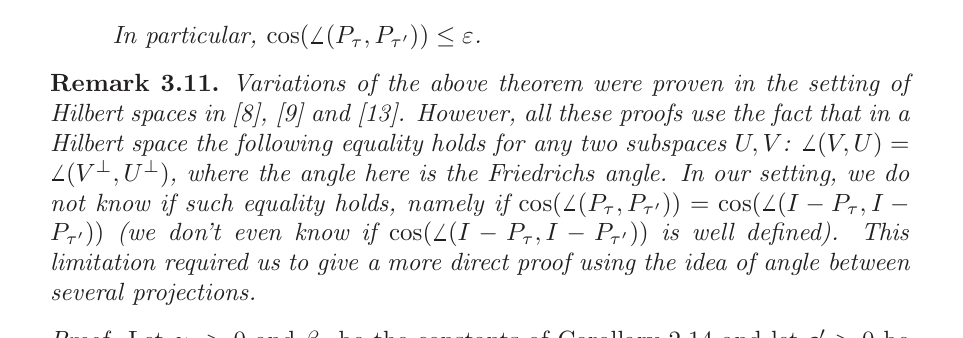
\includegraphics[width=0.88\linewidth]{figures/complement_angle_crop.png}
\end{center}

\section{Idea of the proof}

The definition controls products of the chosen projections, not merely the
angle between their ranges.  If one projection is oblique, its norm can be
larger than one even in a Hilbert space.  Taking the two ranges to be distinct
one-dimensional lines makes their intersection zero, so the required
intersection projection is just the zero map.  The source definition then
reduces to the maximum of two product norms.  One of these products is exactly
the oblique projection, whose Euclidean norm is \(\sqrt 2\).

\section{Counterexample}

\begin{theorem}
\label{thm:cosine-exceeds-one}
There exist a Banach space \(X\), two bounded projections \(P_1,P_2\) on \(X\),
and an admissible projection \(P_{1,2}\) in the sense of Definition 2.10 of
\cite{oppenheim1512}, such that
\[
\cos(\angle(P_1,P_2))>1.
\]
Indeed this value can already be \(\sqrt 2\) on \(X=\mathbb R^2\) with the
Euclidean norm.
\end{theorem}

\begin{proof}
Let \(X=\mathbb R^2\) with its Euclidean norm and define
\[
P_1=
\begin{pmatrix}
1&0\\
0&0
\end{pmatrix},
\qquad
P_2=
\begin{pmatrix}
1&0\\
1&0
\end{pmatrix}.
\]
Equivalently, \(P_1(x,y)=(x,0)\) and \(P_2(x,y)=(x,x)\).  Both maps are
projections, since \(P_1^2=P_1\) and \(P_2^2=P_2\).  Their ranges are
\[
M_1=\operatorname{span}(1,0),
\qquad
M_2=\operatorname{span}(1,1),
\]
and hence \(M_1\cap M_2=\{0\}\).  Thus \(P_{1,2}=0\) is a projection onto the
intersection and satisfies the two required identities
\[
P_{1,2}P_1=P_{1,2},\qquad P_{1,2}P_2=P_{1,2}.
\]

The definition therefore gives
\[
\cos(\angle(P_1,P_2))
=
\max\{\|P_1P_2\|,\|P_2P_1\|\}.
\]
Now \(P_1P_2=P_1\), so \(\|P_1P_2\|=1\), while \(P_2P_1=P_2\).  The map
\(P_2\) is the rank-one operator \(e_1^\ast\otimes(1,1)\), and its Euclidean
operator norm is
\[
\|P_2\|=\|e_1^\ast\|\,\|(1,1)\|=\sqrt2.
\]
Consequently
\[
\cos(\angle(P_1,P_2))=\sqrt2>1.
\]
\end{proof}

\begin{proposition}
\label{prop:complements-not-defined}
For the same \(P_1,P_2\), the source definition of
\(\cos(\angle(I-P_1,I-P_2))\) is not applicable: there is no projection onto
\(\operatorname{im}(I-P_1)\cap\operatorname{im}(I-P_2)\) satisfying the two
compatibility identities required in Definition 2.10.
\end{proposition}

\begin{proof}
Put
\[
Q_1=I-P_1=
\begin{pmatrix}
0&0\\
0&1
\end{pmatrix},
\qquad
Q_2=I-P_2=
\begin{pmatrix}
0&0\\
-1&1
\end{pmatrix}.
\]
Both \(Q_1\) and \(Q_2\) are projections and both have range
\(\operatorname{span}(0,1)\).  Hence the relevant intersection is again
\(\operatorname{span}(0,1)\).

Every projection \(R\) onto this line has the form
\[
R_c=
\begin{pmatrix}
0&0\\
c&1
\end{pmatrix}
\]
for some scalar \(c\).  If \(RQ_1=R\), then applying both sides to \(e_1\)
gives \(0=ce_2\), so \(c=0\).  Thus \(R=Q_1\).  But then
\[
RQ_2=Q_1Q_2=Q_2\neq Q_1=R.
\]
Therefore no such \(R\) can satisfy both \(RQ_1=R\) and \(RQ_2=R\), so the
angle between the complementary projections is not well defined under the
source definition.
\end{proof}

\section{Verification notes}

The example is finite dimensional, and all identities are exact matrix
identities.  The included script
\texttt{code/rank\_two\_projection\_angle\_check.py} verifies the idempotence,
the product norms, and the obstruction to the complementary intersection
projection.  The value \(\sqrt2\) is exact; the numerical output is only a
sanity check.

\section{Novelty and limitations}

Local run indexes were searched for arXiv:1512.08188, the title, and the core
keywords ``angle between projections'', ``Friedrichs angle'', and ``averaged
projections''; no exact prior packet or attempt was found.  Bounded web
searches on June 28, 2026 for exact phrases around
\(\cos(\angle(P_1,P_2))\leq 1\), Oppenheim's projection-angle cosine, and
arXiv:1512.08188 plus ``angle between projections'' found no separate
literature answer beyond the source arXiv record.

The example does not challenge the theorems in \cite{oppenheim1512}, which
assume small numerical bounds on the defined cosine when they use it.  It only
settles the two general definitional questions raised in Remarks 2.11 and 3.11:
the quantity need not be bounded by one, and complement angles need not be
defined for arbitrary bounded projections.

\section{Human-review recommendation}

The key point for review is whether Definition 2.10 is intended to allow
arbitrary bounded projections, including non-orthogonal projections on a
Hilbert space.  The surrounding text says ``projection'' in the Banach-space
sense \(P^2=P\), so the example appears to be a literal counterexample to the
general question in Remark 2.11.

\begin{thebibliography}{9}
\bibitem{oppenheim1512}
I. Oppenheim,
\emph{Vanishing of cohomology with coefficients in representations on Banach
spaces of groups acting on Buildings},
arXiv:1512.08188v2, 2016.
\url{https://arxiv.org/abs/1512.08188}.
\end{thebibliography}

\end{document}
